\documentclass[UTF8]{ctexart}
\usepackage{amsmath,amssymb,booktabs,graphicx,geometry}
\geometry{a4paper,margin=2.4cm}
\graphicspath{{figures/}}
\title{有效人口规模 $N_{\rm eff}$ 下的单阈值控制敏感性实验}
\author{}
\date{\today}

\begin{document}
\maketitle

\section{问题和模型口径}
原始西安实验取 $N=13,163,000$。这个口径对应全市人口下的均匀混合近似。
若传播主要发生在有限接触网络中，可以把 SIQR 方程中的归一化尺度解释为有效混合人口
$N_{\rm eff}$。本实验不改变控制律结构，只考察 $N_{\rm eff}$ 改变后，
阈值控制的启动时间和平台期长度如何变化。

感染项写为
\[
\frac{\beta c(t)(1-q(t))S(t)I(t)}{N_{\rm eff}}.
\]
对每个 $N_{\rm eff}$，固定 $\beta,\gamma,\delta_q,c(t),q(t)$，只重新拟合初始种子
$I_0$，并令 $S_0=N_{\rm eff}-I_0$、$R(0)=0$。这个设定是条件性敏感性分析，
不是重新估计全部传播参数。

\section{实验设计}
扫描
\[
N_{\rm eff}\in\{5\times10^4,10^5,3\times10^5,10^6,3\times10^6,13,163,000\}.
\]
阈值采用三种口径：
\[
\eta=100,\qquad \eta=520,\qquad \eta=0.002N_{\rm eff}.
\]
其中 $\eta=0.002N_{\rm eff}$ 用于观察同比例缩放；$\eta=100,520$ 用于观察固定绝对阈值时
$\eta/N_{\rm eff}$ 随 $N_{\rm eff}$ 下降而增大的影响。

\section{数值结果}
表中 $\Delta t=t_2-t_1$ 表示平台控制时长，主成本 $J$ 使用 $w_c=1,w_q=2$。

\begin{tabular}{cccccccc}
\toprule
$N_{\rm eff}$ & 阈值口径 & $\eta$ & $\hat I_0$ & $t_1$ & $\Delta t$ & $T_{\rm clear}$ & $J$ \\
\midrule
50000 & $\eta=100$ & 100 & 1.3086e-03 & 11.13 & 85.07 & 176.20 & 40.25 \\
1e+05 & $\eta=100$ & 100 & 1.1424e-03 & 11.26 & 170.63 & 292.64 & 81.68 \\
3e+05 & $\eta=100$ & 100 & 1.0484e-03 & 11.34 & 512.86 & 711.96 & 247.12 \\
1e+06 & $\eta=100$ & 100 & 1.0182e-03 & 11.37 & 1710.66 & 2060.37 & 826.03 \\
3e+06 & $\eta=100$ & 100 & 1.0098e-03 & 11.38 & 5132.94 & 5726.47 & 2480.00 \\
1e+07 & $\eta=100$ & 100 & 1.0066e-03 & 11.38 & 22523.29 & 23748.32 & 10884.65 \\
50000 & $\eta=520$ & 520 & 1.3086e-03 & 12.82 & 15.95 & 78.60 & 7.26 \\
1e+05 & $\eta=520$ & 520 & 1.1424e-03 & 12.92 & 32.41 & 112.08 & 15.27 \\
3e+05 & $\eta=520$ & 520 & 1.0484e-03 & 12.98 & 98.23 & 220.78 & 47.12 \\
1e+06 & $\eta=520$ & 520 & 1.0182e-03 & 13.00 & 328.58 & 535.26 & 158.46 \\
3e+06 & $\eta=520$ & 520 & 1.0098e-03 & 13.01 & 986.71 & 1329.75 & 475.93 \\
1e+07 & $\eta=520$ & 520 & 1.0066e-03 & 13.01 & 4331.01 & 5027.38 & 2092.21 \\
50000 & $\eta=0.002N_{\rm eff}$ & 100 & 1.3086e-03 & 11.13 & 85.07 & 176.20 & 40.25 \\
1e+05 & $\eta=0.002N_{\rm eff}$ & 200 & 1.1424e-03 & 11.95 & 85.07 & 186.51 & 40.74 \\
3e+05 & $\eta=0.002N_{\rm eff}$ & 600 & 1.0484e-03 & 13.12 & 85.07 & 202.70 & 40.25 \\
1e+06 & $\eta=0.002N_{\rm eff}$ & 2000 & 1.0182e-03 & 14.34 & 85.07 & 220.36 & 40.38 \\
3e+06 & $\eta=0.002N_{\rm eff}$ & 6000 & 1.0098e-03 & 15.44 & 85.07 & 236.46 & 40.43 \\
1e+07 & $\eta=0.002N_{\rm eff}$ & 26326 & 1.0066e-03 & 16.90 & 85.07 & 258.11 & 40.71 \\
\bottomrule
\end{tabular}


\begin{figure}[htbp]
\centering
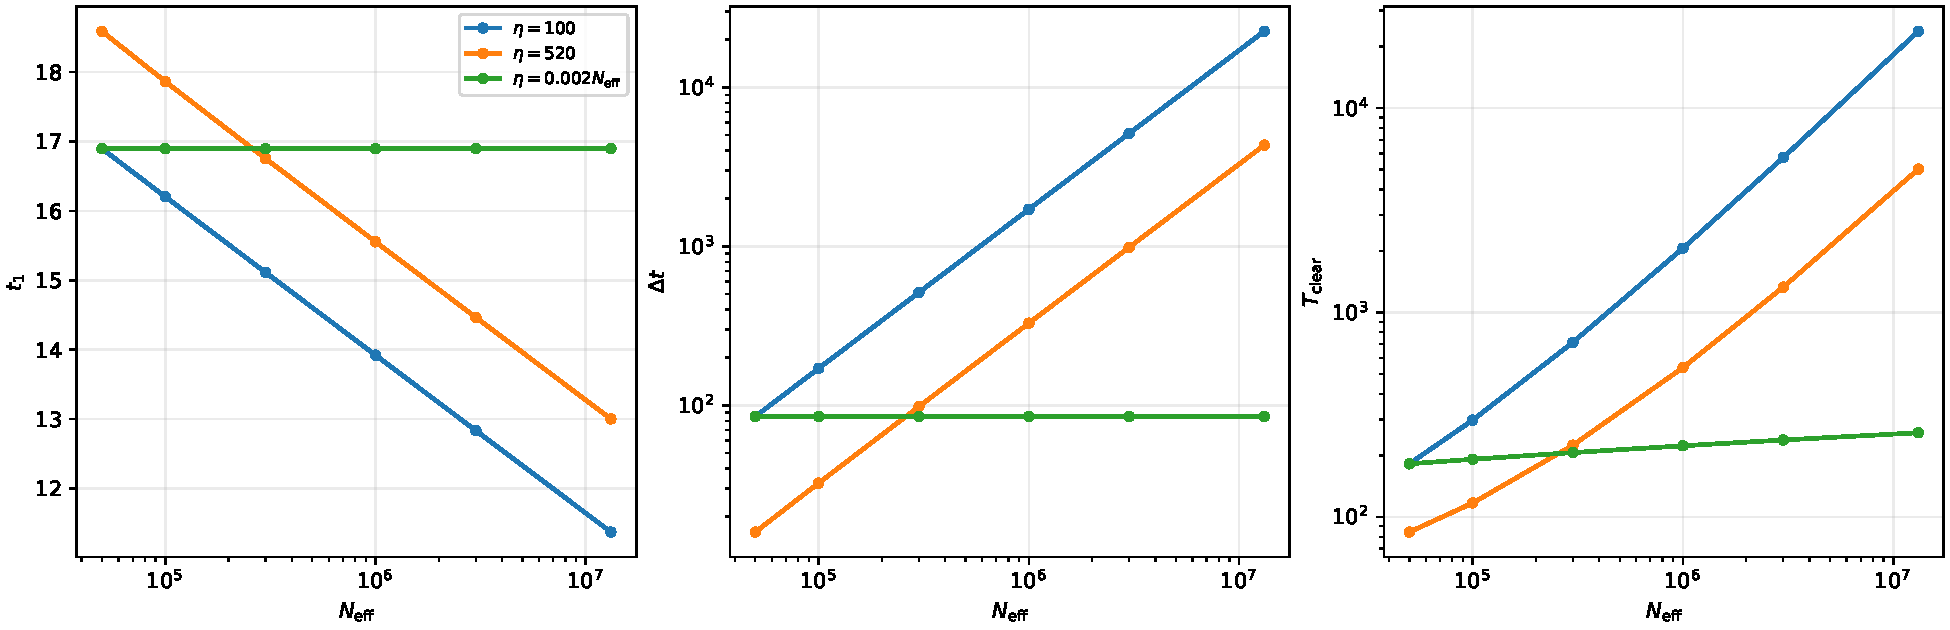
\includegraphics[width=0.95\linewidth]{effective_population_time_metrics.pdf}
\caption{不同 $N_{\rm eff}$ 下的 $t_1$、$\Delta t$ 和 $T_{\rm clear}$。}
\end{figure}

\begin{figure}[htbp]
\centering
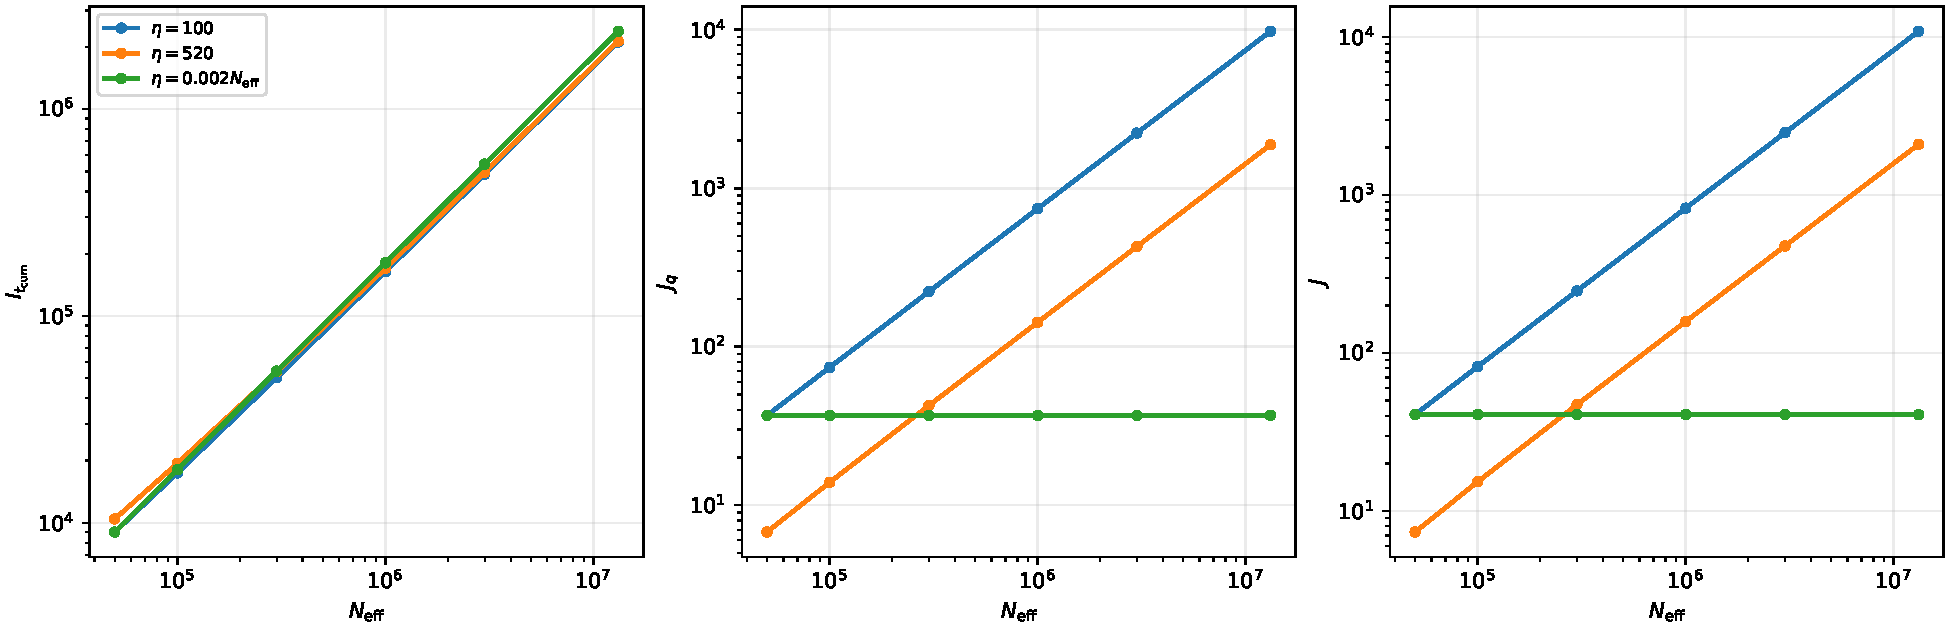
\includegraphics[width=0.95\linewidth]{effective_population_cost_metrics.pdf}
\caption{不同 $N_{\rm eff}$ 下的累计感染和控制成本指标。}
\end{figure}

\begin{figure}[htbp]
\centering
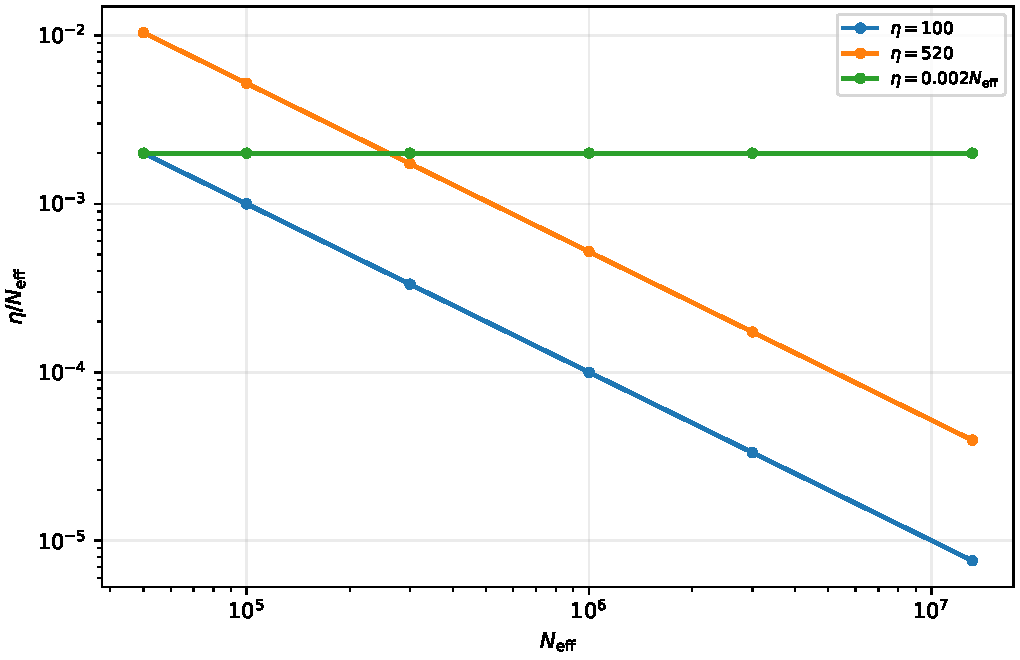
\includegraphics[width=0.68\linewidth]{effective_population_eta_fraction.pdf}
\caption{三类阈值口径对应的 $\eta/N_{\rm eff}$。}
\end{figure}

\section{初步观察}
在当前固定传播参数的设定下，$N_{\rm eff}=13,163,000$ 且
$\eta=0.002N_{\rm eff}$ 时，计算得到
\[
t_1\approx 16.90,\qquad
\Delta t\approx 85.07,\qquad
T_{\rm clear}\approx 258.11.
\]
这与原西安主基准属于同一数量级。

当固定绝对阈值 $\eta=100$ 时，若从 $N_{\rm eff}=13,163,000$ 降到
$N_{\rm eff}=50,000$，$\eta/N_{\rm eff}$ 增大，平台期由
\[
\Delta t\approx 22523.29
\]
变为
\[
\Delta t\approx 85.07.
\]
这一变化对应的是阈值相对有效人口比例的改变，而不是阈值控制律本身的改变。

\section{限制}
本实验固定 $\beta,\gamma,\delta_q,c(t),q(t)$，只重新拟合 $I_0$。因此结果只能解释为：
在给定传播参数和控制函数下，$N_{\rm eff}$ 作为有效混合人口尺度如何影响阈值控制指标。
若要把某个 $N_{\rm eff}$ 解释为真实传播网络规模，还需要空间活动、接触网络或分区病例数据支持，
并可能需要重新估计 $\beta$ 或控制函数。

\end{document}
